% Normative RIGHT decision model -- from pub_rse_methodology/goldstandard_uml.tex
% The figure* float, caption and \ref{} cross-references were removed so the
% picture can stand alone; the \ref targets became plain text.
\documentclass[tikz,border=6pt]{standalone}
% Shared preamble for the standalone renders of the RIGHT-framework figures.
% The tikz styles are copied verbatim from pub_rse_methodology/uml_shapes.tex so
% that the standalone PDFs look exactly like the ones in the paper.
\usepackage[utf8]{inputenc}
\usepackage[T1]{fontenc}
\usepackage{graphicx}
\usepackage{times}
\usepackage{amssymb}
\usepackage{xcolor}
\usepackage{tikz}
\usetikzlibrary{arrows.meta,positioning,shapes.geometric,shapes.misc,calc}

\tikzset {
    initial/.style={circle, fill=black, minimum size=5mm, inner sep=0pt},
    action/.style={draw, rounded corners=2pt, minimum width=28mm,
        minimum height=8mm, align=center},
    decision/.style={draw, diamond, aspect=2, minimum height=8mm,
        minimum width=8mm, inner sep=1pt, align=center},
    fork/.style={draw, fill=black, minimum width=20mm, minimum height=4mm},
    vfork/.style={draw, fill=black, minimum width=2mm, minimum height=14mm},
    box/.style={draw, rounded corners=2mm, thick, minimum width=18mm,
        minimum height=8mm, align=center},
    rsepic/.style={inner sep=0pt, outer sep=2pt},
    dependency/.style={dashed, <->},
    node distance=8mm,
    uml_activity/.style={draw, line width=0.6pt,
        -{Straight Barb[angle=40:5pt 5]}},
    >=Latex,
    every path/.style={uml_activity}
}

\newcommand{\terminus}{
\includegraphics[height=6mm]{uml_endnode.png}}
\newcommand{\rsecycle}{
\includegraphics[height=12mm]{rse-cycle.png}}

\begin{document}
    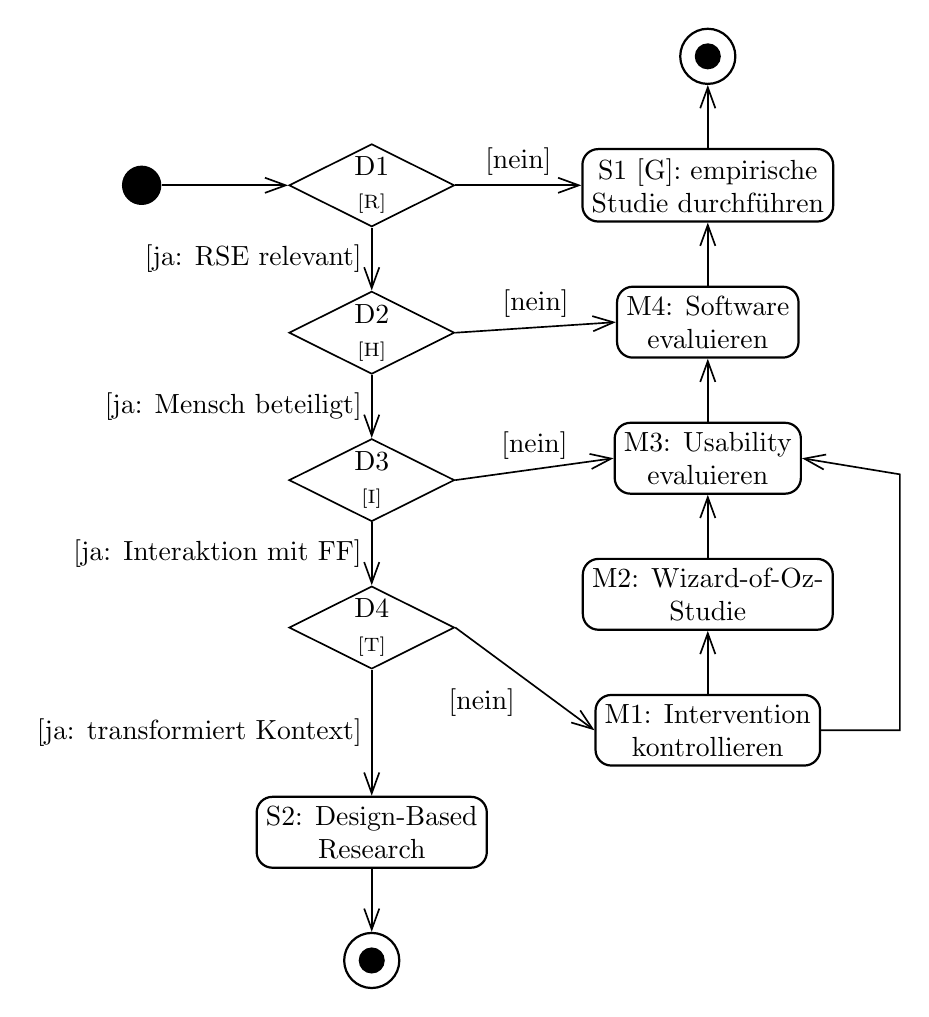
\begin{tikzpicture}[
        final/.style={circle, draw, line width=0.8pt, minimum size=7mm,
            inner sep=0pt},
        node distance=8mm and 16mm,
    ]

        \node[initial] (start) {};

        \node[decision, right=of start] (isRSE) {D1\\{\scriptsize[R]}};
        \node[decision, below=of isRSE] (isHuman) {D2\\{\scriptsize[H]}};
        \node[decision, below=of isHuman] (interactsWithRQ) {D3\\{\scriptsize[I]}};
        \node[decision, below=of interactsWithRQ] (transformsRQ) {D4\\{\scriptsize[T]}};

        \node[box, right=of isRSE] (conductStudy) {S1 [G]: empirische\\Studie durchführen};
        \node[box, below=of conductStudy] (evaluateSoftware) {M4: Software\\evaluieren};
        \node[box, below=of evaluateSoftware] (evaluateUsability) {M3: Usability\\evaluieren};
        \node[box, below=of evaluateUsability] (softwareEffectStudy) {M2: Wizard-of-Oz-\\Studie};

        \node[box, below=of transformsRQ, yshift=-8mm] (dbr) {S2: Design-Based\\Research};
        \node[box, below=of softwareEffectStudy] (noStimulusControl) {M1: Intervention\\kontrollieren};

        \node[final, below=of dbr] (end1) {};
        \node[final, above=of conductStudy] (end2) {};

        \node[circle, fill=black, minimum size=3mm] at (end1.center) {};
        \node[circle, fill=black, minimum size=3mm] at (end2.center) {};

        \draw(start) -- (isRSE);

        \draw (isRSE.east) -- node[midway, above]{[nein]} (conductStudy.west);
        \draw (isHuman.east) -- node[midway, above]{[nein]} (evaluateSoftware.west);
        \draw (interactsWithRQ.east) -- node[midway, above]{[nein]} (evaluateUsability.west);

        \draw (isRSE.south) --
            node[midway, left]{[ja: RSE relevant]} (isHuman.north);
        \draw (isHuman.south) --
            node[midway, left]{[ja: Mensch beteiligt]} (interactsWithRQ.north);
        \draw (interactsWithRQ.south) --
            node[midway, left]{[ja: Interaktion mit FF]} (transformsRQ.north);

        \draw (transformsRQ.south) --
            node[midway, left]{[ja: transformiert Kontext]} (dbr.north);
        \draw (transformsRQ.east) --
            node[midway, below left]{[nein]} (noStimulusControl.west);

        \draw (evaluateSoftware.north) -- (conductStudy.south);
        \draw (evaluateUsability.north) -- (evaluateSoftware.south);
        \draw (softwareEffectStudy.north) -- (evaluateUsability.south);

        \draw (noStimulusControl.north) -- (softwareEffectStudy.south);
        \draw (noStimulusControl.east) -- ++(1,0) -- ++(0,3.25) -- (evaluateUsability.east);

        \draw (conductStudy) -- (end2);
        \draw (dbr) -- (end1);

    \end{tikzpicture}
\end{document}
